\documentclass{report}

\usepackage[utf8]{inputenc}
\usepackage{gensymb}
\usepackage{hyperref}
\usepackage{etoolbox}
\usepackage{graphicx}
\usepackage{geometry}
\usepackage{xifthen}
\usepackage{float}
\usepackage{ulem}
\edef\restoreparindent{\parindent=\the\parindent\relax}
\usepackage[parfill]{parskip}
\restoreparindent
\usepackage{indentfirst}

\title{Developer's Guide}
\author{BERQUEZ Fabien  (1800325), LOGUT Adrien (1815142) \\ \& NAMALGAMUWA Chathura (1815118)}
\date{Updated on 19/02/2016}

\newboolean{all}
\newboolean{lab1}
\newboolean{lab2}
\newboolean{lab3}
\newboolean{fun}

\setboolean{all}{false}
\setboolean{lab1}{false}
\setboolean{lab2}{false}
\setboolean{lab3}{true}
\setboolean{fun}{false}


\begin{document}
\maketitle

\tableofcontents

\newtoggle{diag}

\toggletrue{diag}
%\togglefalse{paper}

\ifthenelse{\boolean{lab1} \OR \boolean{lab2} \OR \boolean{all}}{

\chapter{Preliminary note on the update}

\ifthenelse{\boolean{lab1} \OR \boolean{all}}{
This Developer's Guide has been updated after the first time we submitted the assignment. All the changes made are listed with a comparison in the update section of this guide (the last section), with the explanation of why we did these changes to the initial work.
}

\ifthenelse{\boolean{lab2} \OR \boolean{all}}{
This Developer's Guide has been updated after the first time we submitted the assignment. All the changes made are listed with a comparison in the update section of this guide (the last section), with the explanation of why we did these changes to the initial work. \textbf{Important:} The \hyperref[Usage::lab2] {usage section} has been updated. Please take those modifications into account.
}

}

\chapter{Introduction}

\ifthenelse{\boolean{fun}}{Hi there ! Welcome to the developer's guide of \textbf{arch-LOG8430}.}{This is the developer's guide for \textbf{arch-LOG8430}.} \\

This project was developed for the \href{http://www.polymtl.ca/etudes/cours/details.php?sigle=LOG8430}{Software Architecture} course (LOG8430) at Ecole Polytechnique de Montréal. The course teacher is Yann-Gaël Guéhéneuc and the laboratory teacher is Fábio Petrillo. \\

We are three French exchange students; Fabien Berquez coming from \href{http://www.supelec.fr/374_p_14603/welcome.html}{Supélec} and Adrien Logut and Chathura Namalgamuwa coming from \href{http://ensimag.grenoble-inp.fr/welcome/}{ENSIMAG}. Fabien is a master's student in computer engineering, research-based, whereas Adrien and Chathura are master's students in computer engineering, professional-based. \\ 

\ \\

Note : We advise you to use a \textit{real} pdf reader (and not the one integrated to your web browser for instance) as there are a lot of clickable links that might not be displayed otherwise.
\chapter{Presentation}

You can find all complete assignments (in French) in the \textit{assignment} folder. The objective of this project is to create a multi-platform web music player (eg. Soundcloud, Spotify, etc.) in Java. The source code of this project and all its documentation are available on \href{https://github.com/cnamal/arch-LOG8430}{GitHub}.

\ifthenelse{\boolean{lab1} \OR \boolean{all}}{
\ifthenelse{\boolean{all}}{
\section{Laboratory n$\degree$1}}

The first laboratory's objective is to create a basis for the whole project. A basic music player has to be implemented, using at least 3 web services. \\

We started with implementing a service for Soundcloud because it was the easiest. Indeed, Soundcloud's Web API can be used without authentication. It allowed us to test the code really quickly just using a \textit{client\_id}.}

\ifthenelse{\boolean{lab2} \OR \boolean{all}}{
\ifthenelse{\boolean{all}}{
\section{Laboratory n$\degree$2}}

The second laboratory's objective was to create an RCP application of the first project. \ifthenelse{\boolean{fun}}{\scriptsize \textit{The reason for such a project still eludes us.} \normalsize}}

\section{Laboratory n$\degree$3}
The third laboratory's objective was to create a server that would serve as an interface for all the streaming services. The previous laboratories' applications would serve as clients.

\section{Requirements}

\ifthenelse{\boolean{lab1} \OR \boolean{all}}{
\ifthenelse{\boolean{all}}{
\subsection{Laboratory n$\degree$1}}

\begin{enumerate}
\item Java 8 (Oracle)
\item Git
\item Mac/Linux : maven
\item (optional) e(fx)clipse for Eclipse
\item (optional) ObjectAid for Eclipse
\end{enumerate}

We decide to use maven because early on we knew we were going to use external libraries -especially \href{http://www.javazoom.net/javalayer/javalayer.html}{JLayer}- and using maven is \textit{way} simpler.}

\ifthenelse{\boolean{lab2} \OR \boolean{all}}{
\ifthenelse{\boolean{all}}{
\subsection{Laboratory n$\degree$2}}

\begin{enumerate}
\item Java 8 (Oracle)
\item Git
\item e(fx)clipse for Eclipse
\item Eclipse Plug-in Development Environment
\item (optional) ObjectAid for Eclipse
\end{enumerate}

\ \\
To install e(fx)clipse :

\begin{itemize}
\item Open Eclipse
\item Help -\textgreater Install New Software...
\item If in the list of \textit{Work with} you already have \textit{http://download.eclipse.org/releases/mars} please skip the next step
\item Click on Add and enter \textit{Mars} as the name and \textit{http://download.eclipse.org/releases/mars} as the location
\item Select the \textit{http://download.eclipse.org/releases/mars} location
\item In the text filter, type ``e(" you should see e(fx)clipse come up. Install it.
\end{itemize}

Please follow the same steps to install Eclipse Plug-in Development Environment, but instead of typing ``e(" in the last step, please type ``Plug".
}

\ifthenelse{\boolean{lab3} \OR \boolean{all}}{
\ifthenelse{\boolean{all}}{
\subsection{Laboratory n$\degree$3}}
The requirements are the same as the union of Laboratory n$\degree$1 and n$\degree$2.
}

\section{Usage}

\ifthenelse{\boolean{lab1} \OR \boolean{all}}{
\ifthenelse{\boolean{all}}{
\subsection{Laboratory n$\degree$1}}

\subsubsection{Linux}

\begin{enumerate}
\item Clone the \href{https://github.com/cnamal/arch-LOG8430}{repository}
\item \textit{cd} in the project folder
\item Run \textbf{mvn install}
\item If you use Eclipse, also run \textbf{mvn eclipse:eclipse}
\item Profit!
\end{enumerate}

\subsubsection{Windows}
\begin{enumerate}
\item Open Eclipse and be sure that Maven and Git are both installed (it should be by default, but we are never cautious enough)
\item Open the Git Perspective (Window/Perspective/Open Perspective/Other/Git)
\item Clone a Git \href{https://github.com/cnamal/arch-LOG8430}{repository}
\item After cloning, in the perspective, unwrap the new arch-LOG8430 item and right-click on Working Directory/Import Projects
\item Import it as General Project
\item Go back into the Java Perspective, Right Click on the new project arch-LOG8430/Configure/Convert to Maven Project 
\item We have got an issue when converting to Maven \emph{could} set the JDK to 1.4. If you have compiler error, Right Click on the project/Properties/Uncheck JDK Compilance and set the compilance level to 1.8.
\end{enumerate}


\subsubsection{Eclipse}
Normally, you shouldn't have any problems using Eclipse if you have installed e(fx)clipse (and done \textbf{mvn eclipse:eclipse} on Mac/Linux). However, if you have any problems, make sure the project is configured to use Java 8 (maven should do that for you).
}

\ifthenelse{\boolean{lab2} \OR \boolean{all}}{
\ifthenelse{\boolean{all}}{
\subsection{Laboratory n$\degree$2}}
\label{Usage::lab2}

\begin{enumerate}
\item Clone the \href{https://github.com/cnamal/arch-LOG8430}{repository}
\item Open Eclipse
\item File -\textgreater New -\textgreater Java Project (if not available, click on other and then find Java Project)
\item Uncheck \textit{Use default location} and Browse the location of \textit{CorePlugin}. Click on Finish. 
\item In the Package Explorer, right click on the CorePlugin project -\textgreater Configure (it's towards the end) -\textgreater Configure to Plug-in projects... -\textgreater Select the project and click on Finish.
\item At this point, Eclipse shouldn't show you errors anymore. If not, please send me an email\ifthenelse{\boolean{fun}}{ or \href{https://twitter.com/cnamalgamuwa}{tweet} me.}{.}
\item Open the \textbf{MANIFEST.MF} in \textit{META-INF}. Add in \textit{Runtime} -\textgreater \textit{ Exported Packages} : 
\begin{itemize}
\item com.namal.arch.models
\item com.namal.arch.models.services
\item com.namal.arch.utils
\end{itemize}
\item In the Package Explorer, right click on the CorePlugin project -\textgreater Build Path -\textgreater Configure Build Path... -\textgreater Order and Export -\textgreater Select Core.jar -\textgreater Ok
\item The application requires a MongoDB server to function for the cross-platform part. The configuration needs to be in the \texttt{resources} folder and be named \textit{config.properties}. Please use \textit{config.properties.dist} as a template (be sure to uncomment the used lines). The address, port and db (database) parameters are mandatory. The user information are optional. A \textit{playlists} and a \textit{services} collection need to be in the database already. \textbf{mongodb://\textless dbuser\textgreater:\textless dbpwd\textgreater@\textless address\textgreater:\textless port\textgreater/\textless db\textgreater}
\item In the Package Explorer, right click on the CorePlugin project -\textgreater Build Path -\textgreater Configure Build Path... -\textgreater Source -\textgreater Add Folder -\textgreater Select resources folder -\textgreater OK -\textgreater OK
\item For each plugin (Soundcloud, etc.) you want to add: Repeat steps 3 to 5.
\item To run, right click on any project (Core or plugin) -\textgreater Run As -\textgreater Eclipse Application. \textbf{Linux users need to see next section before hand.}
\item We have \sout{\hyperref[lim::toolbar]{(for now)}} only a View (by that we mean an Eclipse View) that is basically the same view (as in MVC) as in the first laboratory. To access that view, you have multiple possibilities :
\begin{itemize}
\item Window -\textgreater Show View -\textgreater Other -\textgreater Type Namal and you should find the Namal Audio Plugin View.
\item (faster) Click on Quick Access (in the toolbar) and type Namal. You should find the Namal Audio Plugin View
\item (even faster) \textbf{Ctrl+3} opens the Quick Access. Cf previous point to continue.
\end{itemize}
\item To use our application afterwards, please use the User Guide.
\ifthenelse{\boolean{fun}}{\item Profit!}
\end{enumerate}

\subsubsection{Linux}
JavaFX which is used for our view has some compatibility issues with Linux and GTK3 \ifthenelse{\boolean{fun}}{(\#Oracle anyone?)}. To solve this issue, you need to disable GTK3 when running the Eclipse Application \ifthenelse{\boolean{fun}}{(\textit{fair warning: the resulting Eclipse UI Interface is ugly})}: Right click on any project (Core or plugin) -\textgreater Run As -\textgreater Run Configurations -\textgreater Eclipse Application -\textgreater Environment tab -\textgreater New -\textgreater Set \textit{SWT\_GTK3} as Name and \textit{0} as it's Value. You can then Run the project \ifthenelse{\boolean{fun}}{\href{http://i.imgur.com/l9EHHWA.gif}{smoothly}}{smoothly}.
}

\ifthenelse{\boolean{lab3} \OR \boolean{all}}{
\ifthenelse{\boolean{all}}{
\subsection{Laboratory n$\degree$3}}
Using the clients has not changed, except the fact that for the 2nd laboratory RCP client, you only need to do step 1 to 5 - since there aren't any other plugins-.
To launch the server, you will just need to run the Maven command : \textbf{mvn spring-boot:run}.
}

\section{ObjectAid}
ObjectAid is an Eclipse plugin that automatically draws the UML diagrams of your project. If you have installed it, you can use it to open the \textbf{*.ucls} files in the documentation folder.

\chapter{Sequence Diagram}

\ifthenelse{\boolean{lab1} \OR \boolean{all}}{
\ifthenelse{\boolean{all}}{
\section{Laboratory n$\degree$1}}

The figures \ref{play} and \ref{search} are  play sequence and a search sequence respectively.
\iftoggle{diag}{
\begin{figure}[H]

  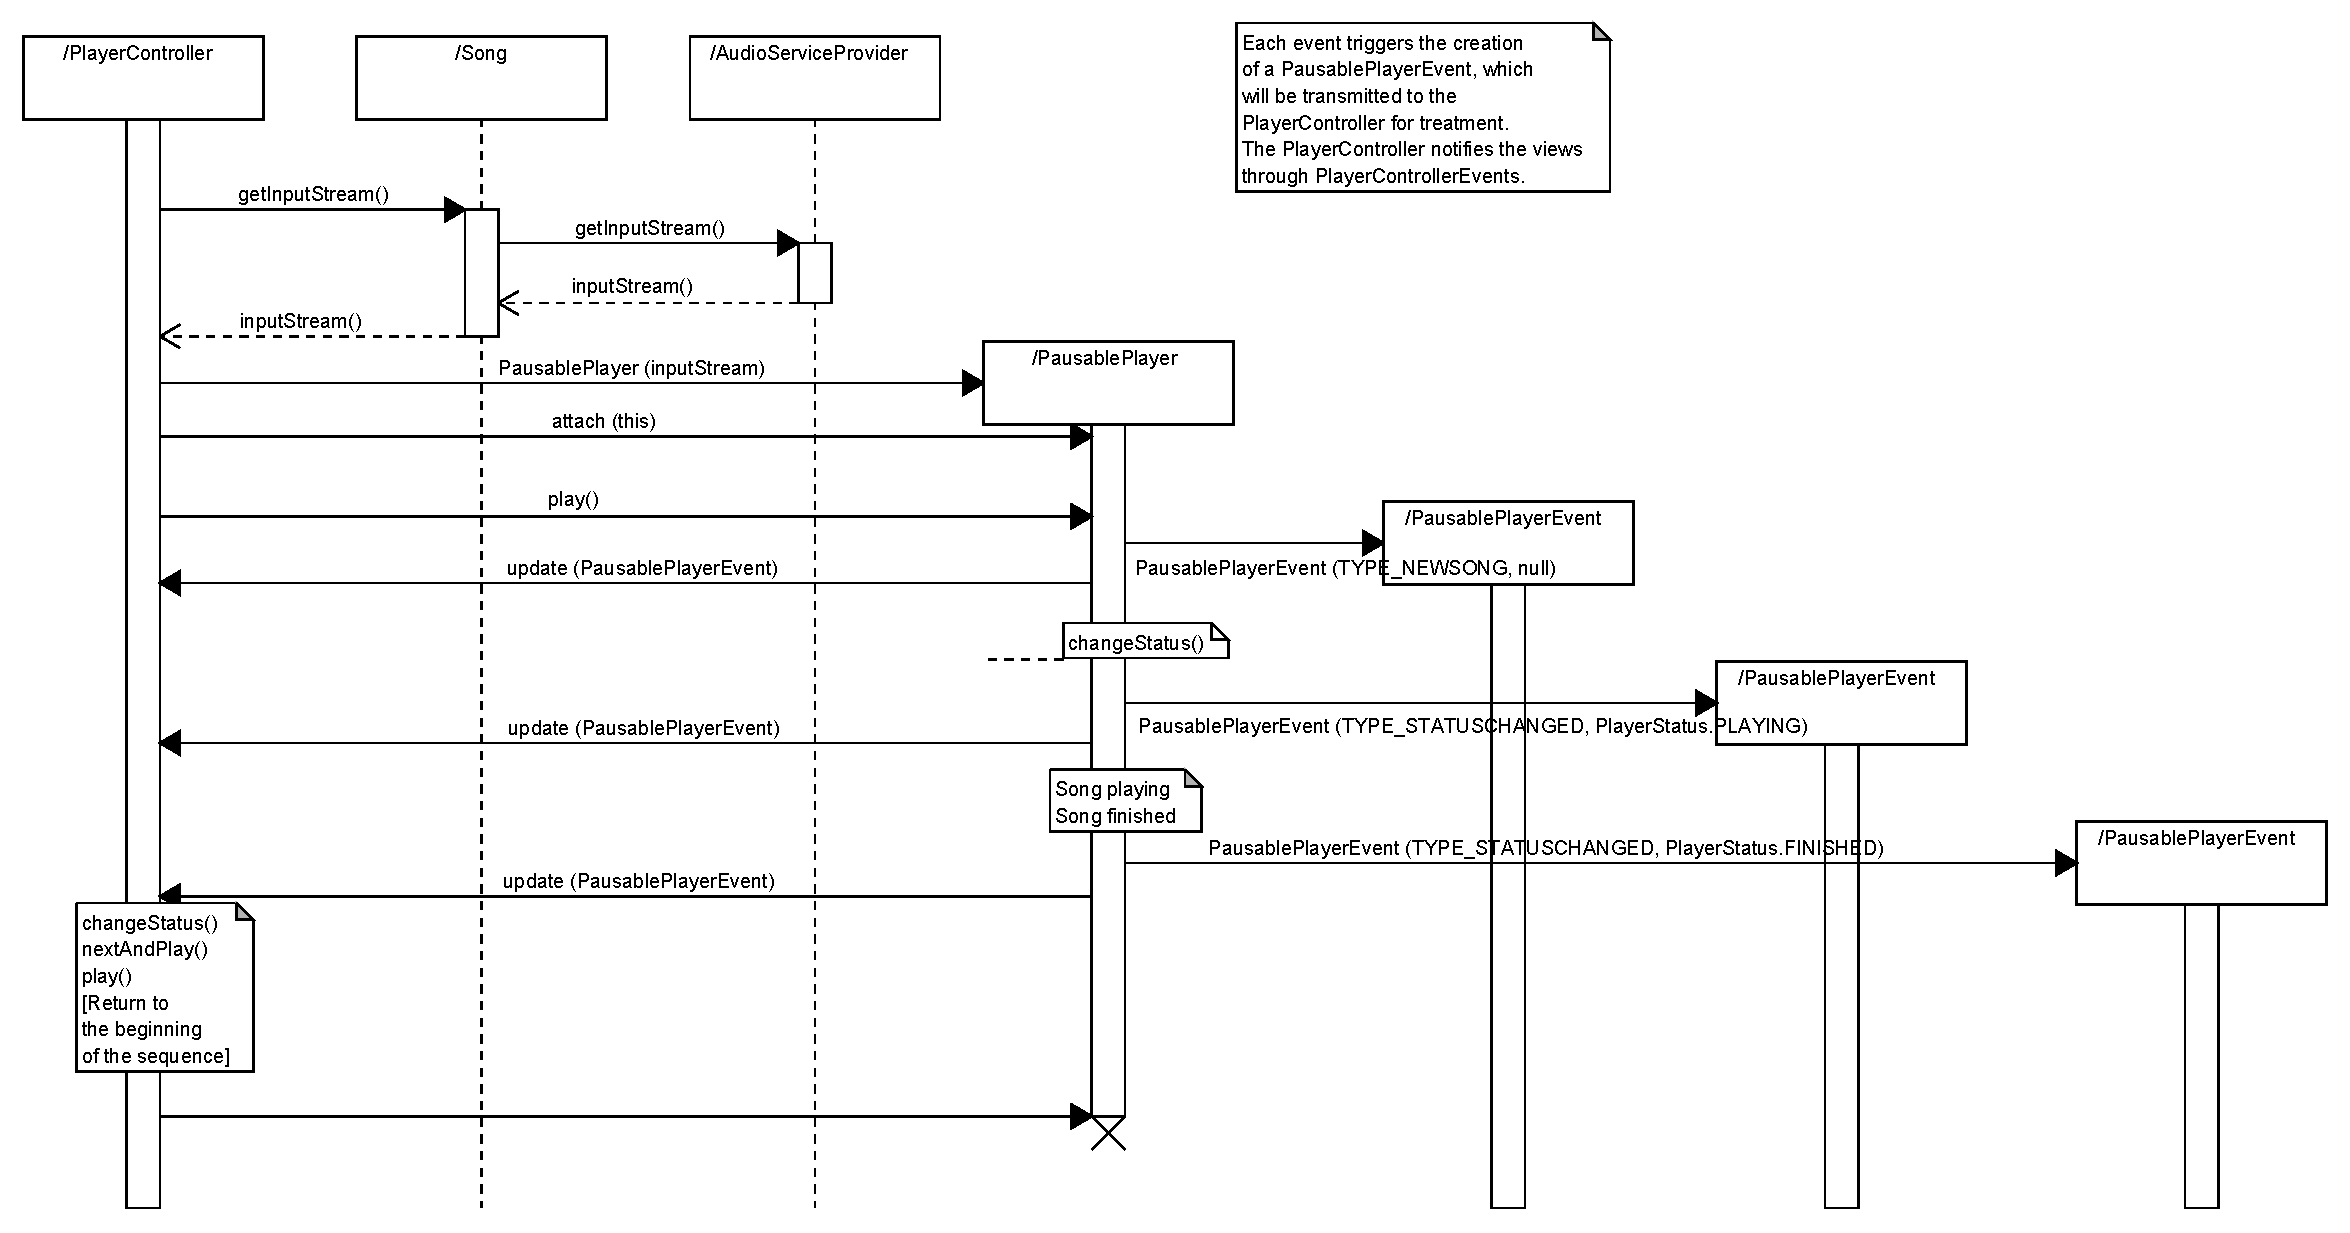
\includegraphics[scale=0.4]{seq/PlaySequence.pdf}
  \caption{Play sequence}
  \label{play}
\end{figure}

\begin{figure}[H]

  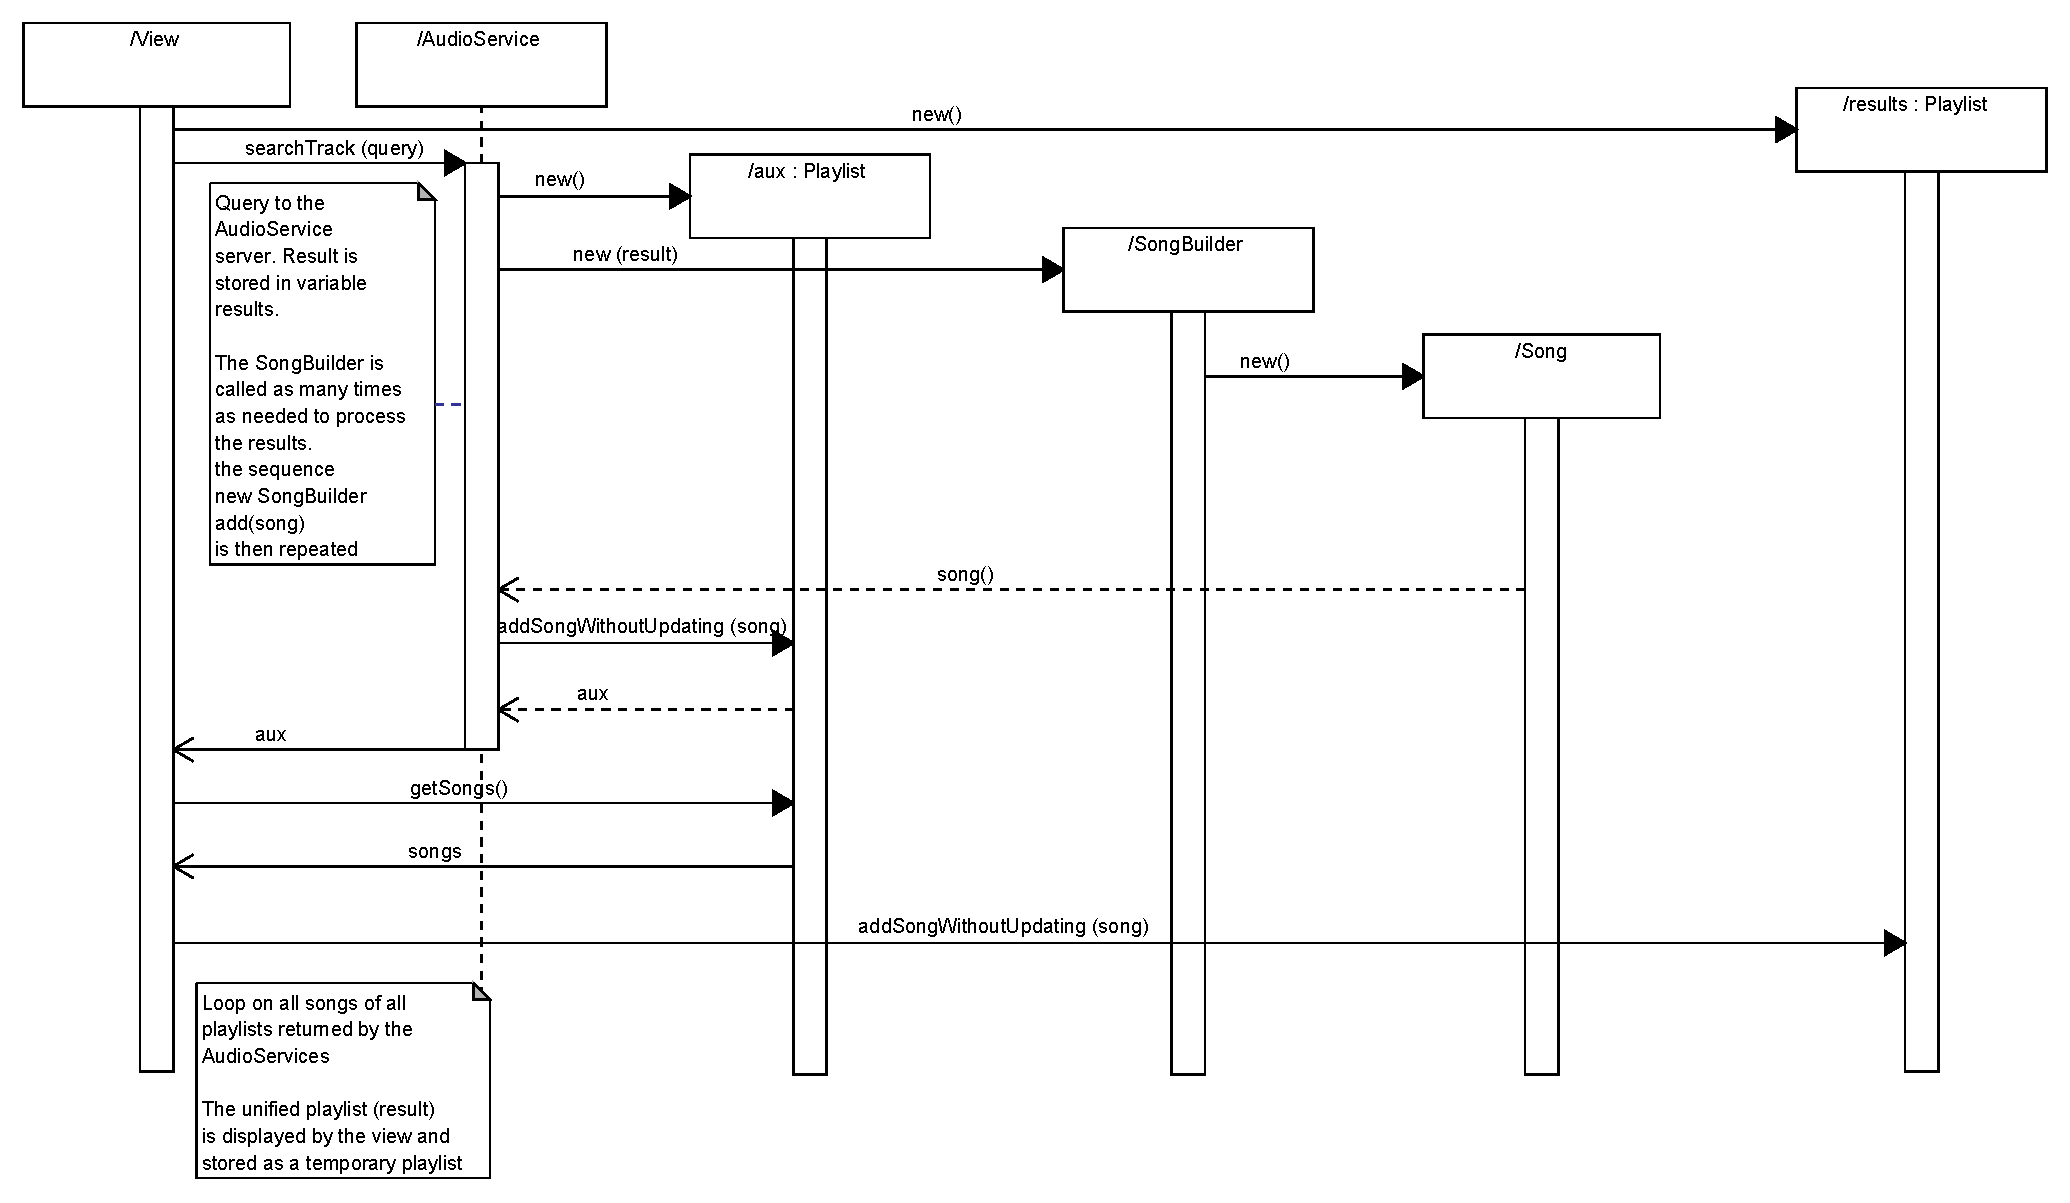
\includegraphics[scale=0.4]{seq/SearchSequence.pdf}
  \caption{Search sequence}
  \label{search}
\end{figure}
}
}
\ifthenelse{\boolean{lab2} \OR \boolean{all}}{
\ifthenelse{\boolean{all}}{
\section{Laboratory n$\degree$2}}

The figures \ref{play2} and \ref{search2} are  play sequence and a search sequence respectively. The classes described are in the CorePlugin jar, created using the first laboratory.

\begin{figure}[H]

  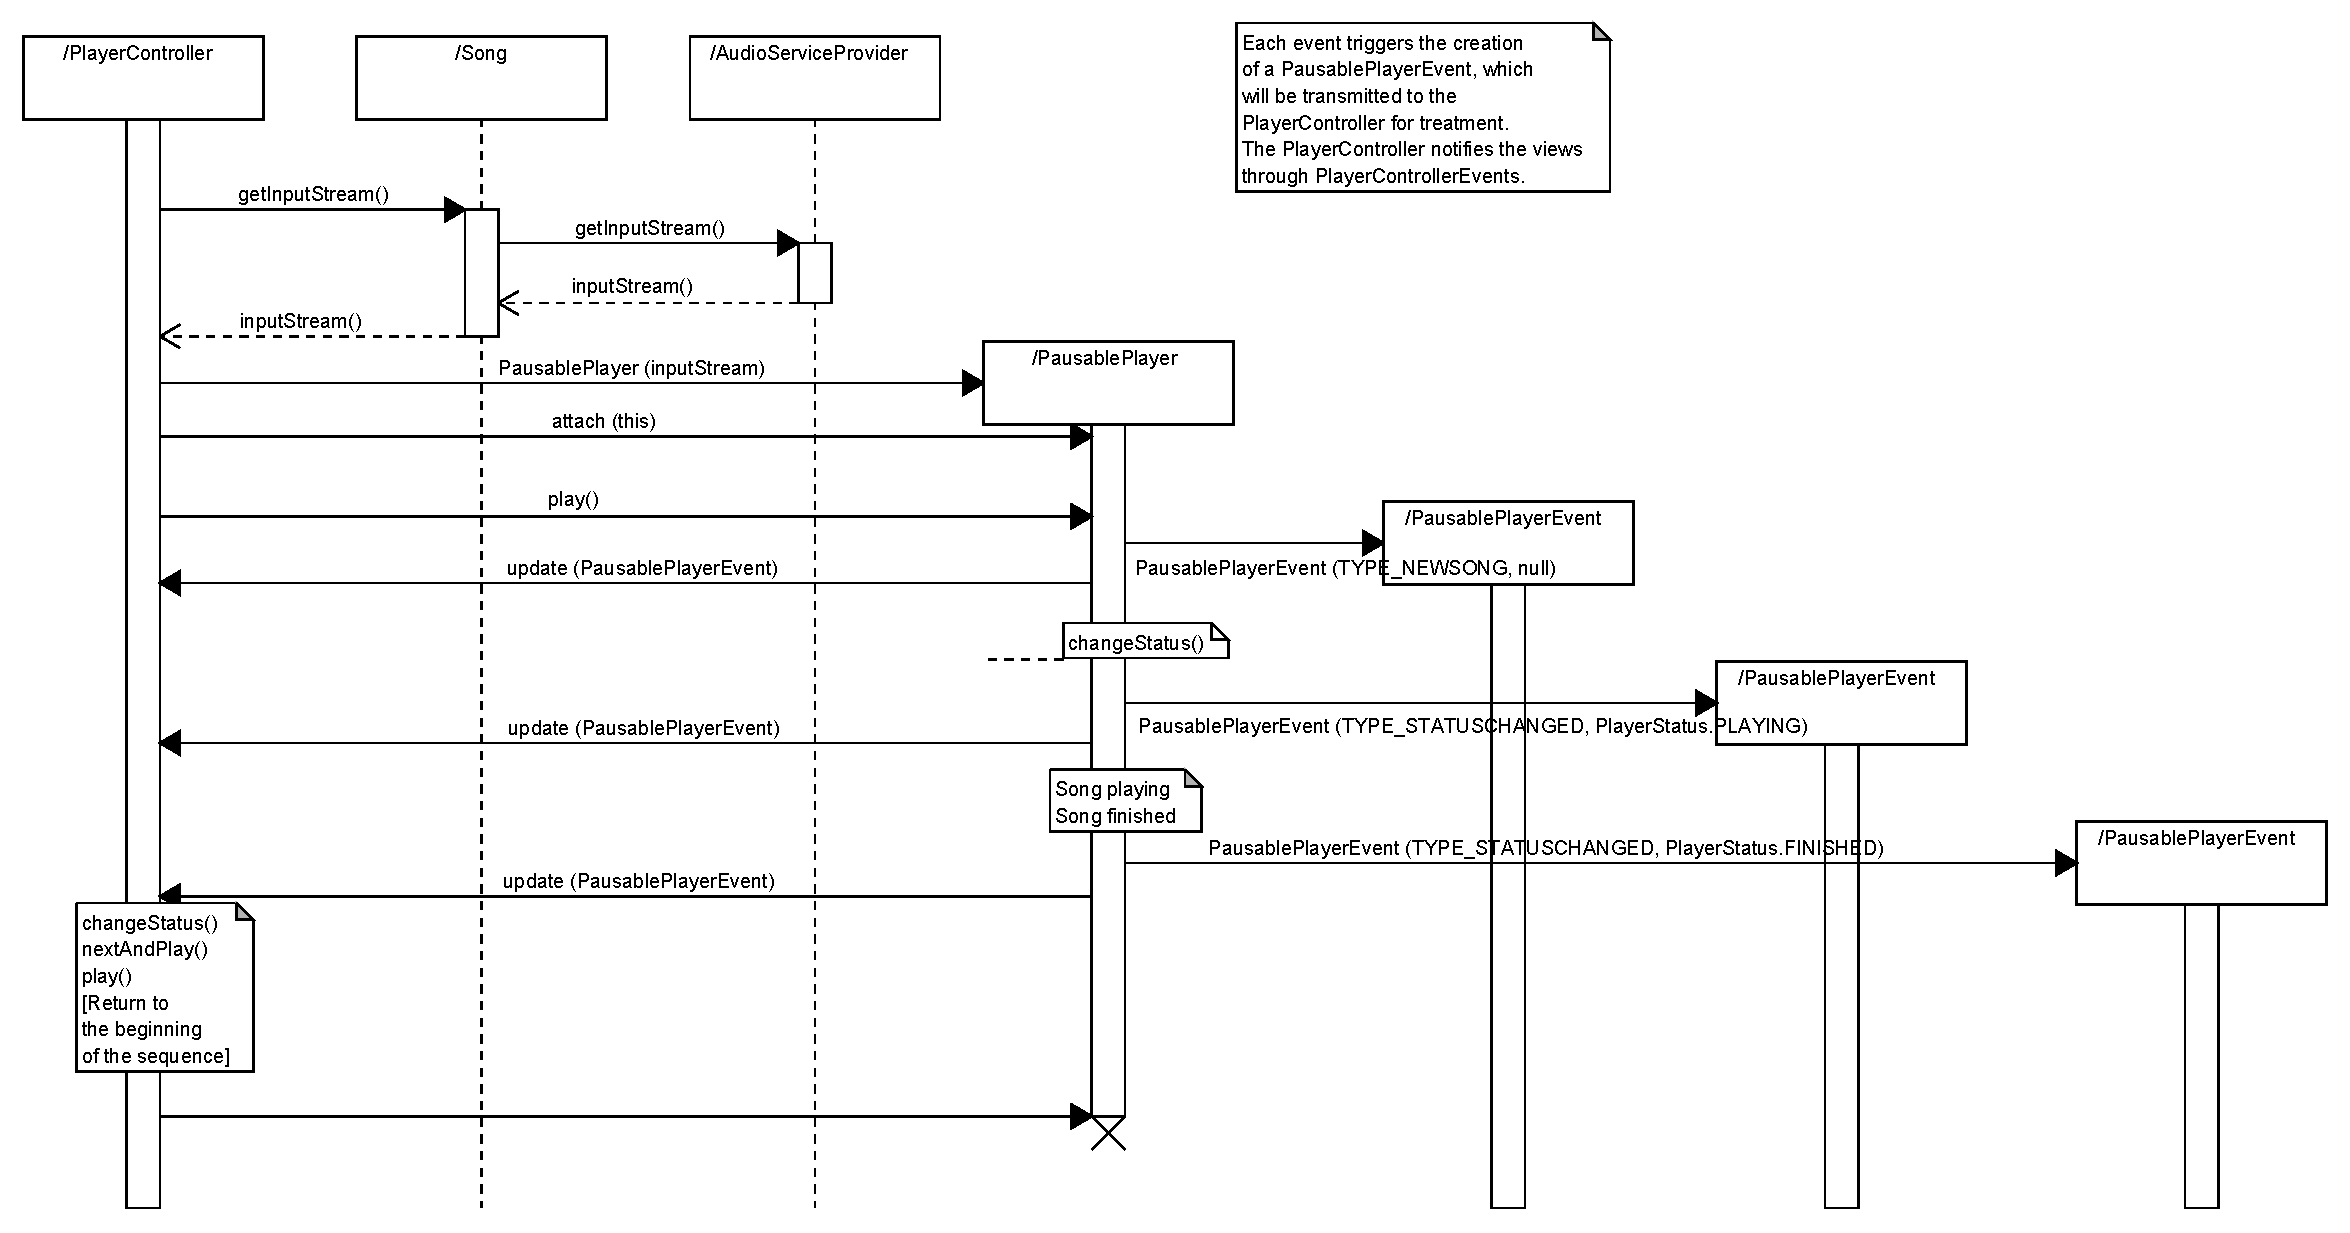
\includegraphics[scale=0.4]{seq/PlaySequence.pdf}
  \caption{Play sequence}
  \label{play2}
\end{figure}

\begin{figure}[H]

  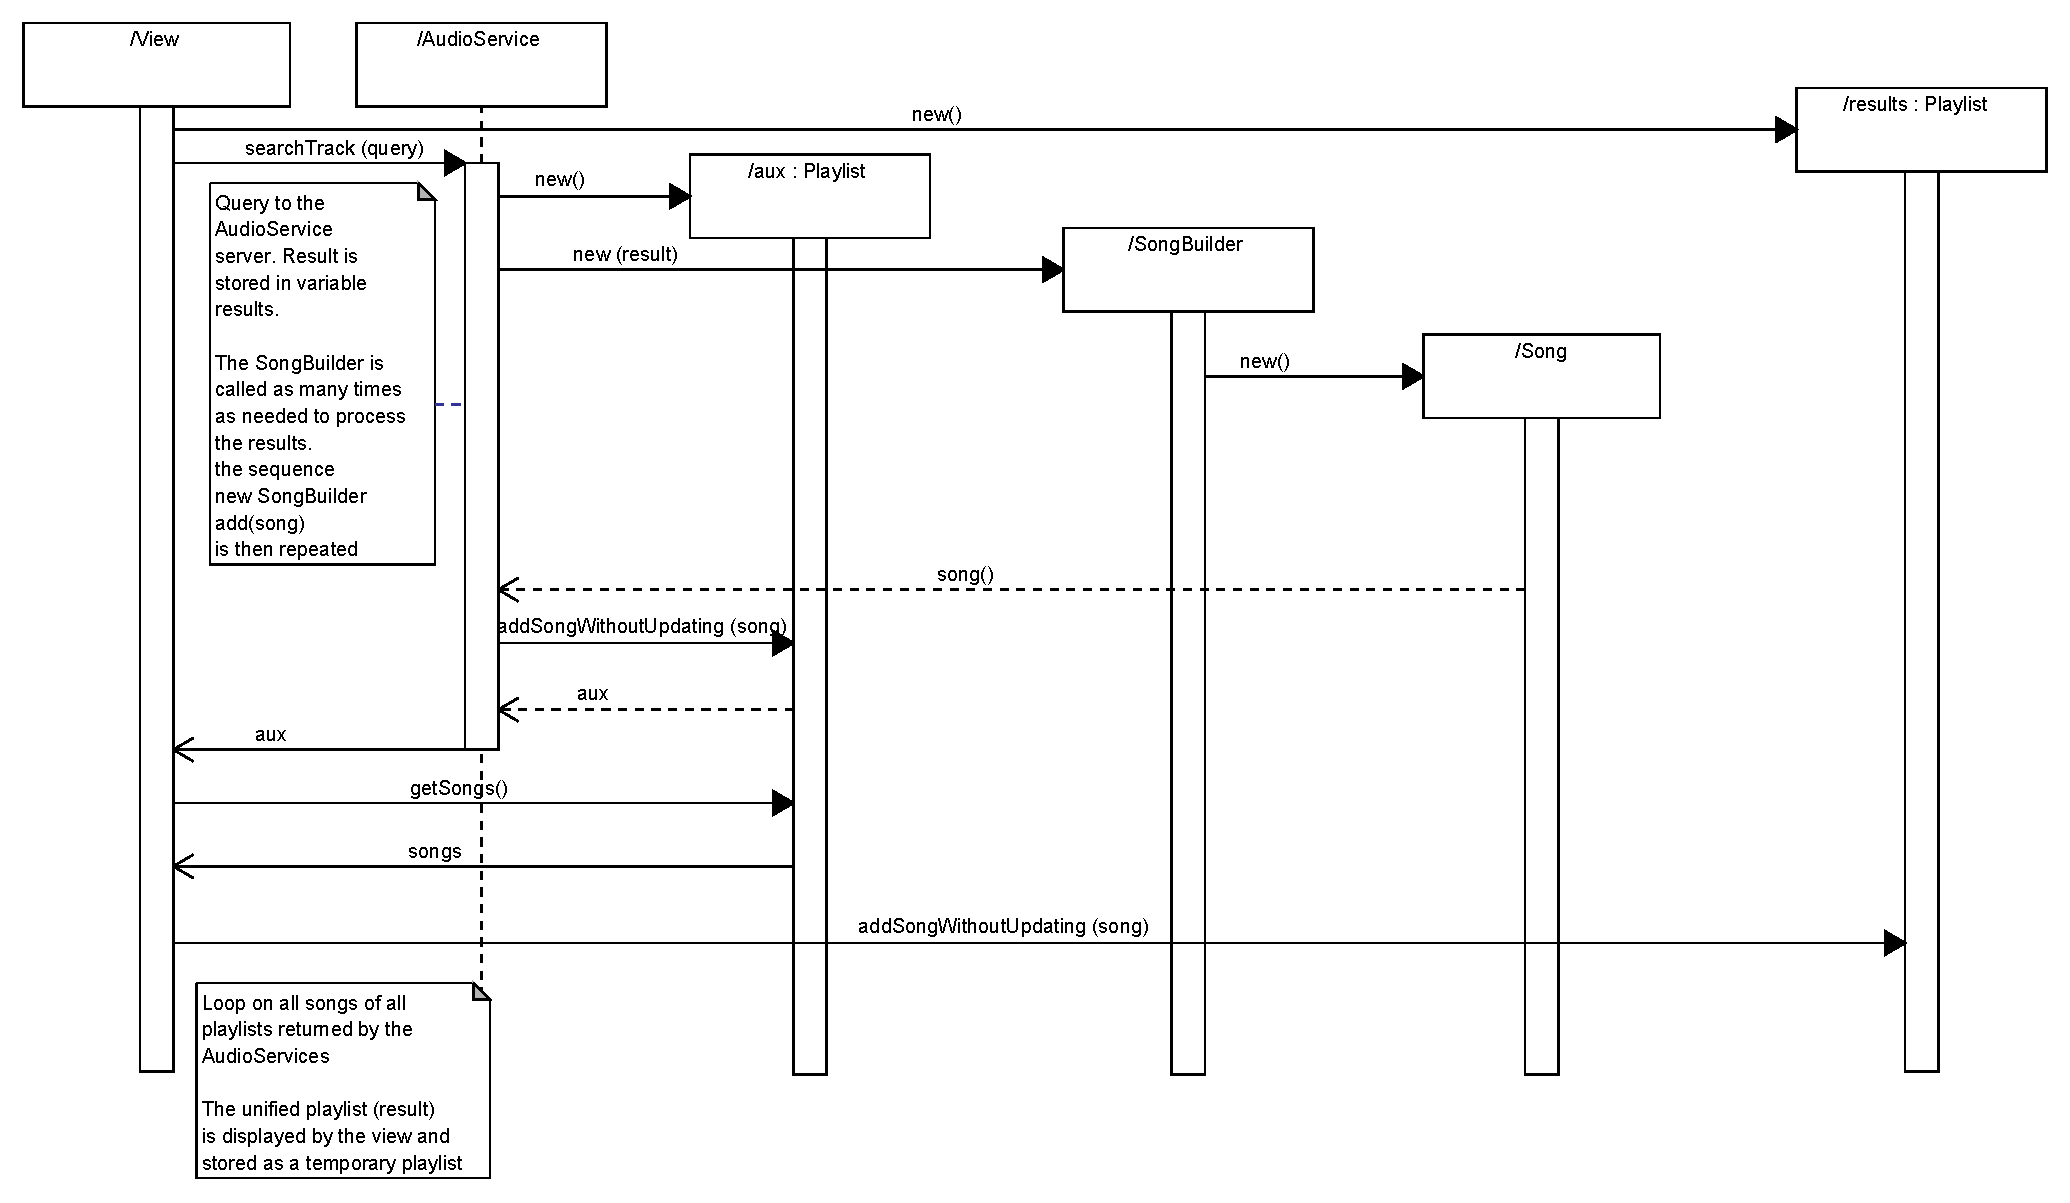
\includegraphics[scale=0.4]{seq/SearchSequence.pdf}
  \caption{Search sequence}
  \label{search2}
\end{figure}

}

\ifthenelse{\boolean{lab3} \OR \boolean{all}}{
\ifthenelse{\boolean{all}}{
\section{Laboratory n$\degree$3}}

\subsection{Clients}
%TODO
\subsection{Server}
Since the sequence diagram isn't pertinent here, we give the full API description. You can view the API by going to the \href{http://editor.swagger.io/}{Swagger editor} and uploading the \textit{swagger.yaml} in \textbf{doc} folder (File -\textgreater Import File).
}

\chapter{Class Diagram}

\ifthenelse{\boolean{lab1} \OR \boolean{all}}{
\ifthenelse{\boolean{all}}{
\section{Laboratory n$\degree$1}}
\subsection{Methodology}

When we chose to do this option (two project options were given), we started to think about the \href{https://s3.amazonaws.com/applause-devmktg/2015/12/02/57kz3goral_YOU_DONT_SAY.png}{architecture of the project}. We started to draw a few UML diagrams on a piece of paper highlighting the main models and a few pattern designs we would use. At the end of that mini work-session, we knew we would use a MVC architecture, and as models we would have \textit{Song} and \textit{Playlist}, as controllers we'd have the \textit{Player} and finally we would have \textit{AudioService(s)} that would be generic. To be able to have numerous audio services, the idea to use the \href{https://en.wikipedia.org/wiki/Strategy_pattern}{\textit{strategy pattern}} was most obvious. However, after this first session, we never drew a UML diagram again. Indeed, the rest of the architecture was designed directly by coding the classes (cf \href{https://github.com/cnamal/arch-LOG8430/commit/d4953e0fc8fc3a7a8641dd7cacef69496f3ca011}{initial commit}). By coding the classes, we mean that every class was created along with it's methods and attributes, but the methods were not implemented. A few \texttt{TODO}s were added to explain what a method should do, and hence explain the main workflow.\\

This way of working has had a lot of advantages but also a few drawbacks (from least to most pertinent): 
\begin{enumerate}
\item \textbf{Advantages}
\begin{itemize}
\item Less boring. Even though this might appear as a joke, it isn't \tiny{(okay maybe a bit)}.\normalsize  However, directly coding gives better sense of progress. The \textit{boring} task of drawing UMLs is replaced by a more fun activity with more or less the same effect. 
\item More productivity. The fact that the exercise is now "fun" makes you want to code more and thus gain in productivity.
\item Kill two birds with one stone. If we had drawn UML diagrams we would have needed to \textit{transcribe} it in Java classes. Granted, it isn't the longest task.
\item Somehow easier. Directly coding allows to find a few bugs or conception flaws we think we wouldn't have had if we had drawn it. Indeed, you are immersed in the code instead of having a layer of abstraction, that are UML classes. One could however argue that the goal was to learn how to immerse yourself using UMLs. It would be an interesting debate.
\end{itemize}
\item \textbf{Disadvantages}
\begin{itemize}
\item Extracting class diagrams. For this guide, we have to add a few diagram classes and recreating UML diagrams feel more of a step back. However, as good lazy developers, we found an Eclipse plugin that did that for us.
\item We are less prone to creating the \textit{perfect} architecture. Being too immersed in the code gives us even more the desire to start coding. Therefore, we could miss a few conception flaws. This happened with the \texttt{Soundcloud} class (cf \hyperlink{blob}{blob issue})
\item Teamwork is harder. The problem is only one person did the whole architecture and \textbf{then} it was debated with the other team members. Therefore, one person \textit{forces} his point of view on the others. Even though the other have the possibility to object, it requires a greater effort of thinking outside the box.
\end{itemize}

Overall, we feel like the advantages outweighed the disadvantages, and therefore we stick by this choice. It allowed us to have a functional player really quickly.

\end{enumerate}

\subsection{Figures}

The figures \ref{Controller} and \ref{Services} are class diagrams of the Controller package and Services package respectively.

\iftoggle{diag}{
\begin{figure}[H]

  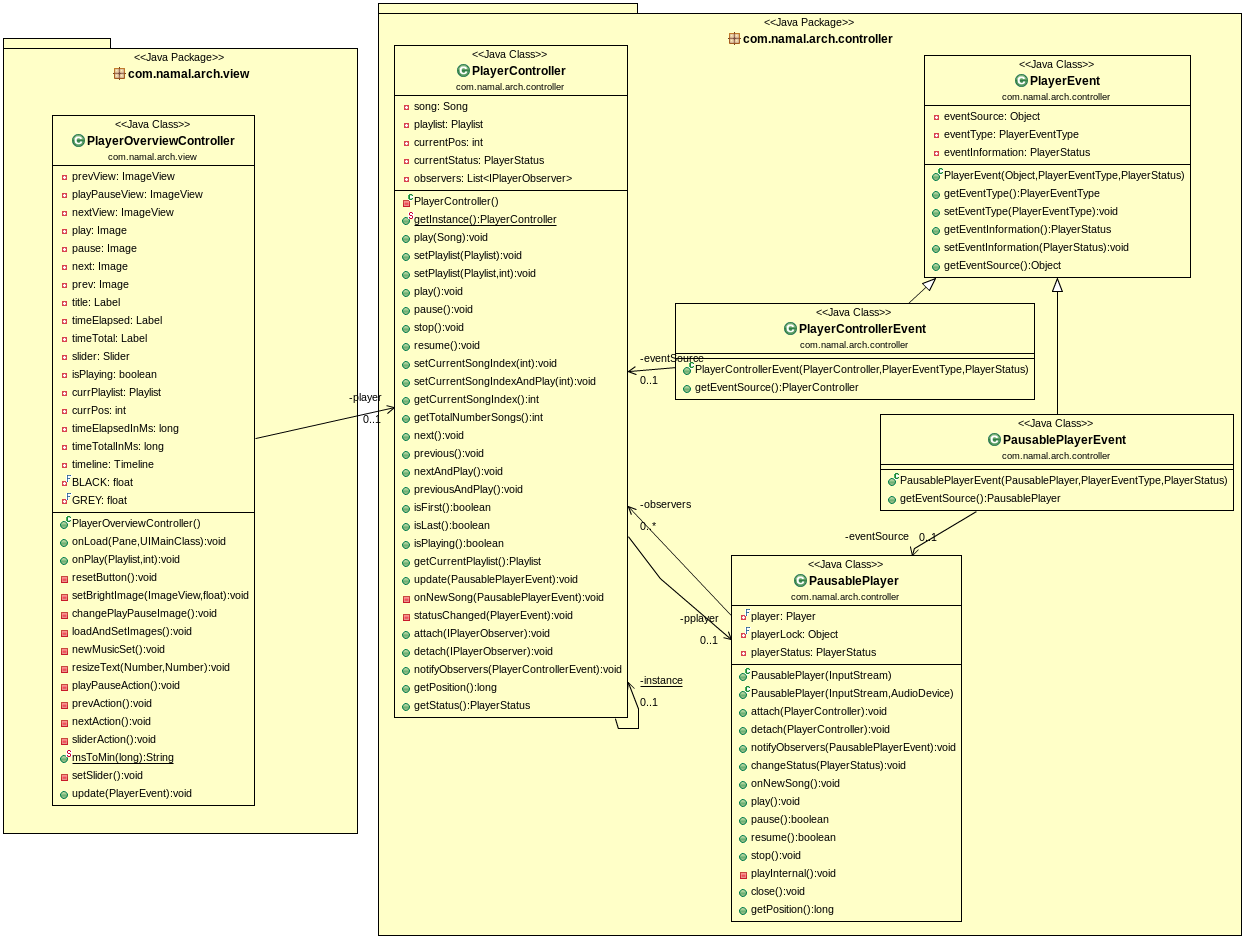
\includegraphics[scale=0.4]{class/Controller.png}
  \caption{Controller package diagram}
  \label{Controller}
\end{figure}

\begin{figure}[H]

  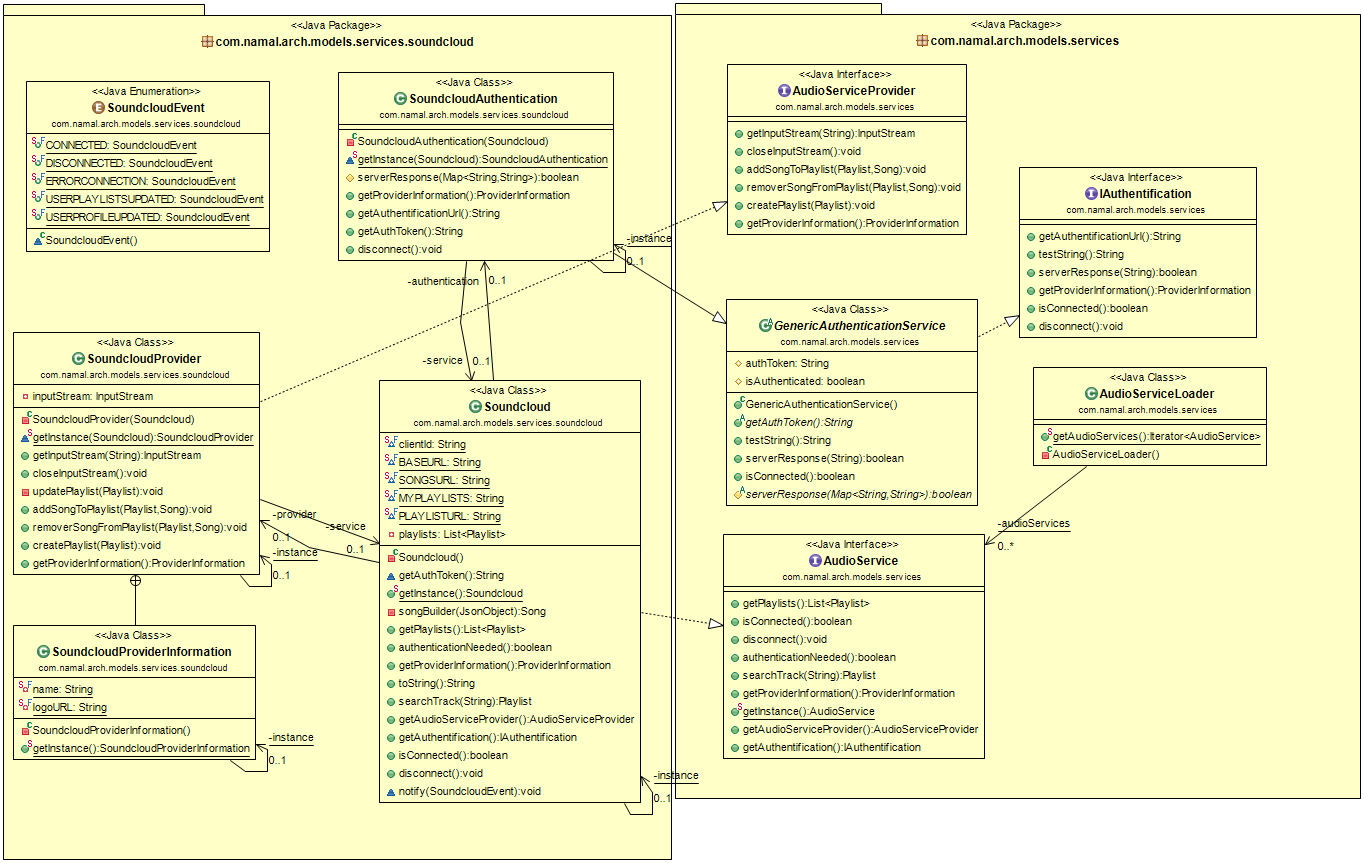
\includegraphics[scale=0.4]{class/Services2.png}
  \caption{Services package diagram}
  \label{Services}
\end{figure}
}

\subsection{Explanations}

\begin{itemize}
\item The MVC architecture allowed us to have a modular project, and everyone worked on a part : Adrien on the view, Fabien on the controller and Chathura on the models/services. 
\item The models have \textit{pure} models and services. This choice is purely aesthetical. The services correspond to the Web services whereas the models correspond to really abstract objects. We could have created only the model package.
\item The \href{https://en.wikipedia.org/wiki/Strategy_pattern}{strategy pattern} allows us to offer an interface for any Audio service. Additionally, one can notice the fact that this pattern allows us to use any type of audio service, whether it is Web-based or your local machine.
\item The \href{https://en.wikipedia.org/wiki/Observer_pattern}{observer pattern} is used as a callback mechanism especially between the view and the controller (\texttt{PlayerController}), but also within the controller (between \texttt{PlayerController} and \texttt{PausablePlayer}). Between the view and the controller, the observer in the \texttt{PlayerController} uses interfaces, since \textit{any} class could want to observe the player. Furthermore, the subject is the \texttt{PlayerController} and not the \texttt{PausablePlayer} because the latter is destroyed/created for every song. We haven't use any interfaces between \texttt{PlayerController} and \texttt{PausablePlayer} since only the \texttt{PlayerController} observes the \texttt{PausablePlayer}.
\item \href{http://weknowmemes.com/generator/uploads/generated/g1406353714448670979.jpg}{Singletons} have been used profusely. It allows us to have only one \textit{entry point} -like the Soundcloud class-, and it solves a lot of potential errors : for example having multiple players could lead to multiple songs being played at the same time, or worse multi-threading issues which would have been very hard to debug. 
\end{itemize}
}

\ifthenelse{\boolean{lab2} \OR \boolean{all}}{
\ifthenelse{\boolean{all}}{
\section{Laboratory n$\degree$2}}

\subsection{Methodology}

The initial goal of the second laboratory was to create an RCP project. \ifthenelse{\boolean{fun}}{However, we found that idea \textit{boring}. Like we said in the presentation, we don't understand the goal of this laboratory; so why not have at least some fun with it?} After discussion with our professor, we were given the green light to create an Eclipse plugin, ie. the service/player is directly integrated to the Eclipse IDE. We did have a few issues to deal with:

\begin{enumerate}
\item Manage to keep the code of the first laboratory. Indeed, Adrien work very hard on the view, to give a good user experience. We didn't want to tell him to code the view again using SWT \ifthenelse{\boolean{fun}}{(which is arguably worst)}. 
\item Manage to make work JavaFX in an Eclipse plugin, especially on Linux.
\item Manage to export the plugin (so that you, \textit{reader}, are able to compile/run the code).
\end{enumerate}

These will be addressed in the Implementation section.

\subsection{Figures}

We completely reused the code of the first laboratory. The only modification made was to have a different ServiceLoader in the first laboratory and the second one. Therefore instead of using a utility AudioServiceLoader, we created an interface which does the same thing. We then have one AudioServiceLoader for the first laboratory and another one for the second laboratory. The view only has an interface.

\begin{center}
\begin{figure}[H]

  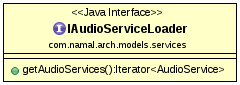
\includegraphics[scale=0.4]{class/AudioServiceLoader.png}
  \caption{Audio service loader interface}
  \label{AudioServiceLoader}
\end{figure}
\end{center}

Otherwise, we only have a few new classes, since the main logic of the application is already in the library. 

\begin{center}
\begin{figure}[H]

  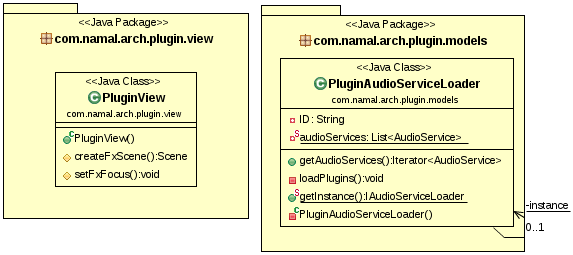
\includegraphics[scale=0.4]{class/Plugin.png}
  \caption{Plugin diagram}
  \label{Plugin}
\end{figure}
\end{center}
}

\ifthenelse{\boolean{lab3} \OR \boolean{all}}{
\ifthenelse{\boolean{all}}{
\section{Laboratory n$\degree$3}}

\subsection{Methodology}

The third laboratory was pretty straight forward, since we were quite familiar with the services. What we decided to do, was to create the API first and implement the server and clients afterwards. This way, we had a \textit{contract} and both implementations could be done separately.

\subsection{Figures}

\subsubsection{Client}
%TODO
\subsubsection{Server}

The previous services interfaces have been slightly modified. 
\begin{center}
\begin{figure}[H]

  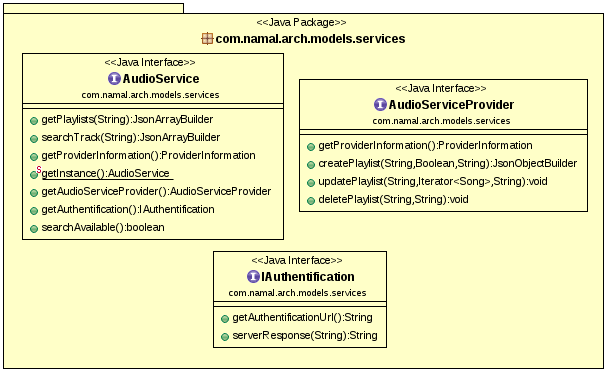
\includegraphics[scale=0.4]{class/servicesServer.png}
  \caption{Services diagram (server)}
  \label{servicesServer}
\end{figure}
\end{center}

The controllers are now the API endpoints :

\begin{center}
\begin{figure}[H]

  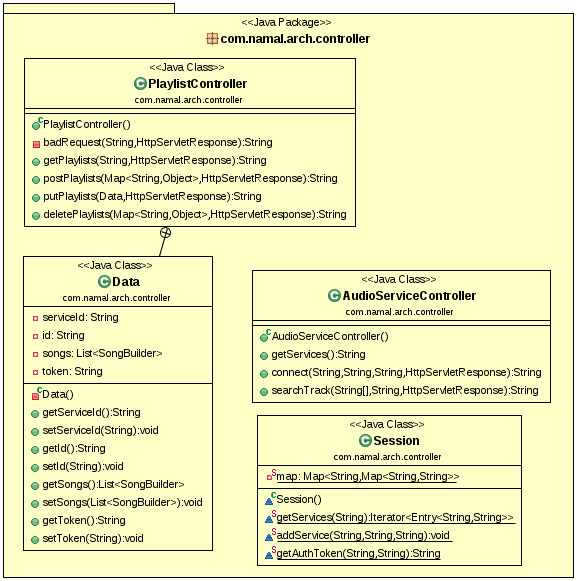
\includegraphics[scale=0.4]{class/controllerServer.png}
  \caption{Controller diagram (server)}
  \label{controllerServer}
\end{figure}
\end{center}

}

\chapter{Implementation}

\ifthenelse{\boolean{lab1} \OR \boolean{all}}{
\ifthenelse{\boolean{all}}{
\section{Laboratory n$\degree$1}}

\subsection{View}
In the MVC model, the view (ie. Graphical User Interface or GUI) is implemented apart the others. GUI was implemented with the pure API Java called JavaFX. 
Everything was implemented in the package view (for Java classes) and the JavaFX resources such as FXML files, CSS files and images are in the folder resources. 

We had the choice between using an GUI (called SceneBuilder) to create our own GUI and save it into FXML files or to code it from scratch in a Java Controller. At the end, both methods were used. In order to organize our view, we used SceneBuilder. And when the view was "repetitive" it was done with Java.

We need for each of or view a controller in order to control our view and react to the user inputs and actions.

\subsubsection{Main UI Class}
The main UI class is essential, everything is loaded from it and each controller has a reference to this class, to interact with other components of the UI. It extends the Application class, used by JavaFX.

\subsubsection{UI Controller}
Each controller of the UI extends the UI Controller which is a simple class with a reference to the UI element(Pane class for JavaFX), and 2 methods used to load a FXML file. Since almost every controller need the FXML loader, it seems it was useful and cleaner to refactor it a parent class.

\subsubsection{Overview Controllers}
The idea here was to create little modules of each function we want to implement instead of a big controller with everything in it. For example, the General Layout, which is the first thing we see is divided in 3 parts. The list at the left, controlled by the controller associated to General Layout, the part top right where the modules from the list will be loaded and the bottom where the player is. Each component is independent and can be loaded where we want. It allows a better maintainability and the possibility to use one module elsewhere without changing anything.

\subsection{Controller}

\subsubsection{Player}

The player we implemented uses the \href{http://www.javazoom.net/javalayer/javalayer.html}{JLayer} library. However, this player had limitations, notably the fact that we couldn't pause the player. We therefore adapted a code found on \href{http://stackoverflow.com/questions/12057214/jlayer-pause-and-resume-song}{Stackoverflow}. It already had a pausing function and the thread handling was already done. The observers and a stopping function were added.

\subsection{Models}

\subsubsection{Bob the builder}
Songs have a lot attributes and worse, some are optional! A solution could have been to have a default constructor with all the mandatory attributes, and setters for all the optional parameters. However, there were still \textit{too many} compulsory attributes. This \href{http://stackoverflow.com/a/40324/5795409}{Stackoverflow answer} offers a neat solution -the articles it refers to are great-. We ended up doing a mix between the source code suggested in the answer and a \href{https://dzone.com/articles/factories-builders-and-fluent-}{\texttt{Fluent interface pattern}}.

\subsubsection{Strategy Pattern}
The main interface is \texttt{AudioService},  and \texttt{AudioServiceProvider} and \texttt{IAuthentification} are just helper interfaces to have a distinct interfaces for distinct parts. It offers a certain modularity. \\
The \texttt{AudioServiceLoader} is a singleton class that acts as a bridge between the view and the services. 
}

\ifthenelse{\boolean{lab2} \OR \boolean{all}}{
\ifthenelse{\boolean{all}}{
\section{Laboratory n$\degree$2}}

\ifthenelse{\boolean{fun}}{\subsection{\href{https://31.media.tumblr.com/tumblr_m6ppniq7uX1r54kwx.gif}{Manage to keep the code of the first laboratory}}}{\subsection{Manage to keep the code of the first laboratory}}
%\subsection{\ifthenelse{\boolean{fun}}{}{}}

We didn't want to change our code of the first laboratory.\ifthenelse{\boolean{fun}}{ Not only did we work hard on it, but w}{ W}e felt like it was a bad practice to copy the code of the first lab\ifthenelse{\boolean{fun}}{ \footnote{``Paradoxical in a software architecture class"(Comment by Chathura Namalgamuwa)}}. Therefore, we decide to use the first project as a library (by creating jars) that would be used by our second project. The main issue was to manage and plug JavaFX in an Eclipse plugin which usually works using SWT.

However, when it finally worked, this was the proof that our previous architecture was quite robust. Only a minor interface was added.

\subsection{Manage to make work JavaFX in an Eclipse plugin}
\label{implem::long}
The lack of documentation and tutorials was the biggest obstacle in this process. Furthermore, when we tried to run JavaFX plugins on Linux, the application would crash, with a Segmentation Fault \ifthenelse{\boolean{fun}}{(yes a SegFault in Java). To simplify our lives, no logs were written. Turns out}{. Indeed}, JavaFX uses GTK2 and SWT GTK3, which creates a conflict resulting in the SegFault. It took approximately 10h to solve all the issues related to JavaFX.

\ifthenelse{\boolean{fun}}{\subsection{\href{http://truegif.com/pictures/gif/4461.gif}{Manage to export the plugin}}}{\subsection{Manage to export the plugin}}

This was the last issue. Indeed, using Maven seemed way too complicated in this laboratory, since there were our dependencies (the jars of the previous laboratory, and all the libraries it depended on) but also the dependencies for eclipse plugin development. Therefore after a lot of trial and error, we came up with the solution given in the \hyperref[Usage::lab2]{Usage section}. This took approximately 3h to solve, and isn't optimal since we aren't using any build automation tool.
}

\ifthenelse{\boolean{lab3} \OR \boolean{all}}{
\ifthenelse{\boolean{all}}{
\section{Laboratory n$\degree$3}}

\subsection{Client}
%TODO
\subsection{Server}

\ifthenelse{\boolean{fun}}{\subsubsection{\href{http://data.whicdn.com/images/33689024/large.gif}{Swagger}}}{\subsubsection{Swagger}}
Swagger was used to create the API but was \textbf{NOT} used to generate the code. We felt that the swagger project, albeit quite promising, wasn't mature enough to create a \textit{good} code. For instance, it is impossible to download the HTML/CSS/JS code of the editor, once the API is written (that is why we give you the yaml and not a generated html directly)\footnote{Link to github issue : \url{https://github.com/swagger-api/swagger-editor/issues/664}}.

\ifthenelse{\boolean{fun}}{\subsubsection{https://www.facebook.com/photo.php?fbid=10209423114439593&set=gm.10153621153678691&type=3&theater}{Spring boot}}{\subsubsection{Spring boot}}

We used Spring boot to develop the server. It is pretty straight forward and easier to use than writing J2EE code directly. However, we had a hard time getting programmatically the address of the server (localhost) and the port (8080). We could have hardcoded those values, but it wouldn't have been modular enough.

}

\chapter{Limitations}

\ifthenelse{\boolean{lab1} \OR \boolean{all}}{
\ifthenelse{\boolean{all}}{
\section{Laboratory n$\degree$1}}

\begin{itemize}
\item The authentication services were rushed towards the end, so they are not perfect. For instance, a failed authentication doesn't throw an exception but only returns false, or if the Soundcloud account is modified (especially if the user's password is modified), the program will not handle it -but shouldn't crash-. The only solution is to \ifthenelse{\boolean{fun}}{\href{http://img.pandawhale.com/post-16780-have-you-tried-forcing-an-unex-uQSY.gif}{disconnect and reconnect}}{disconnect and reconnect}. 
\item Even though they weren't yet implemented, Spotify and Deezer services don't allow third-party apps to stream their music, even if the user is authenticated. Only 30 seconds of the song will be played. Playlist management and song displays should however be functional.
\item Threads are only created for the player. Therefore, any communication with a Web service blocks the main thread.
\item Testing is very hard for this project, hence the lack of tests. Indeed, a lot of testing requires user interaction (even without the view).
\item \hypertarget{db}{The architecture}, \textit{in it's present form}, doesn't work if we want to save the data in a database. For instance, the Song model has a reference to a \texttt{AudioServiceProvider}. This flaw was discovered talking to another group who work on the same project as us. For now, the architecture is good enough for the objectives we fixed ourselves. Furthermore, we don't think the tweaks needed should be too difficult to add.
\end{itemize}
}

\ifthenelse{\boolean{lab2} \OR \boolean{all}}{
\ifthenelse{\boolean{all}}{
\section{Laboratory n$\degree$2}}

\begin{itemize}
\item New
\begin{itemize}
\item We have \hyperref[lim::toolbar]{(for now)} only a View (by that we mean an Eclipse View) that is basically the same view (as in MVC) as in the first laboratory
\item On Linux, you cannot use GTK3.
\end{itemize}
\item Previous
\begin{itemize}

\item The authentication services were rushed towards the end, so they are not perfect. For instance, a failed authentication doesn't throw an exception but only returns false, or if the Soundcloud account is modified (especially if the user's password is modified), the program will not handle it -but shouldn't crash-. The only solution is to \ifthenelse{\boolean{fun}}{\href{http://img.pandawhale.com/post-16780-have-you-tried-forcing-an-unex-uQSY.gif}{disconnect and reconnect}}{disconnect and reconnect}. 
\item Even though they weren't yet implemented, Spotify and Deezer services don't allow third-party apps to stream their music, even if the user is authenticated. Only 30 seconds of the song will be played. Playlist management and song displays should however be functional.
\item Testing is very hard for this project, hence the lack of tests. Indeed, a lot of testing requires user interaction (even without the view).
\item \hypertarget{db}{The architecture}, \textit{in it's present form}, doesn't work if we want to save the data in a database. For instance, the Song model has a reference to a \texttt{AudioServiceProvider}. This flaw was discovered talking to another group who work on the same project as us. For now, the architecture is good enough for the objectives we fixed ourselves. Furthermore, we don't think the tweaks needed should be too difficult to add.
\end{itemize}
\end{itemize}
}


\ifthenelse{\boolean{lab3} \OR \boolean{all}}{
\ifthenelse{\boolean{all}}{
\section{Laboratory n$\degree$3}}

\subsection{Client}
%TODO
\subsection{Server}

\begin{itemize}
\item There is no User system on the cross-platform playlists. Anyone can access/modify/delete anyone's cross-platform playlist. We felt like it wasn't the most important feature.
\item Authentication uses a hack to work. Indeed, in a real system, a service (Soundcloud, Spotify or Deezer) should callback our server once the user has successfully authenticated. However, since our server is running locally, we cannot use that system. Therefore the callback is sent by the client to our server which then process' the service's answer.
\end{itemize}
}

\chapter{Future fixes}

\ifthenelse{\boolean{lab1} \OR \boolean{all}}{
\ifthenelse{\boolean{all}}{
\section{Laboratory n$\degree$1}}


\begin{enumerate}
\item Urgent 
\begin{itemize}
\item \sout{Souncloud has become a \textit{blob} class. We should be able to break the class in different \textit{sub-classes} since the interfaces are already done. The possible issue is if the sub-classes are dependant on each other.}
\item \sout{The authorization process is a bit messy and is currently entirely implemented in the Soundcloud class. However, the authorization process is the same for Souncloud and Spotify (and possibly Deezer), so the code can be refactored in a helper \textit{generic} class.}
\item These changes have been made (cf Update section)
\end{itemize}
\item Intermediate
\begin{itemize}
\item Create cross-platform playlists. Beside the obvious difficulty of the task, the current architecture might need to be slightly \hyperlink{db}{modified}.
\end{itemize}
\item Hopefully
\begin{itemize}
\item Create threads for web queries. This is very complicated and isn't necessarily worth it. Indeed, if you have a good internet connection, the waiting times aren't bad. However, once we will add other services, this might become necessary.
\end{itemize}
\end{enumerate}
}

\ifthenelse{\boolean{lab2} \OR \boolean{all}}{
\ifthenelse{\boolean{all}}{
\section{Laboratory n$\degree$2}}

No new bugs were introduced.

\begin{enumerate}
\item Urgent 
\begin{itemize}
\label{lim::toolbar}
\item \sout{We didn't have \hyperref[implem::long]{time} to add buttons to control the player in the toolbar. A few updates should be made to the player observers (detect that the player is paused for instance). Overall, it shouldn't be too complicated.}
\item \sout{Add new services, namely Spotify and Deezer. It shouldn't take too long.}
\item \sout{Do the Javadoc.}
\end{itemize}
\item Intermediate
\begin{itemize}
\item \sout{Create cross-platform playlists. Beside the obvious difficulty of the task, the current architecture might need to be slightly \hyperlink{db}{modified}.}
\end{itemize}
\end{enumerate}

These changes have been made (cf Update section).
}

\ifthenelse{\boolean{lab3} \OR \boolean{all}}{
\ifthenelse{\boolean{all}}{
\section{Laboratory n$\degree$3}}

\subsection{Client}
%TODO
\subsection{Server}

Hopefully, we will add a User system on our server, for cross-platform playlists. 
}

\ifthenelse{\boolean{lab1} \OR \boolean{lab2} \OR \boolean{all}}{
\chapter{Updates}}

\ifthenelse{\boolean{lab1} \OR \boolean{all}}{
\ifthenelse{\boolean{all}}{
\section{Laboratory n$\degree$1}}

\subsection{Class Diagramm}
\subsubsection{Comparison}
The Class Diagramm has been updated to accurately show the changes made to the architecture of the software between the first and the second edition of this guide. The changes have essentially been made to the services package. The \texttt{Soundcloud} class has been split into several classes, each of whom having a smaller and more precise responsibility, instead of one "God Class". Here are the differences between the two class diagramm for this package :
\iftoggle{diag}{
\begin{figure}[H]

  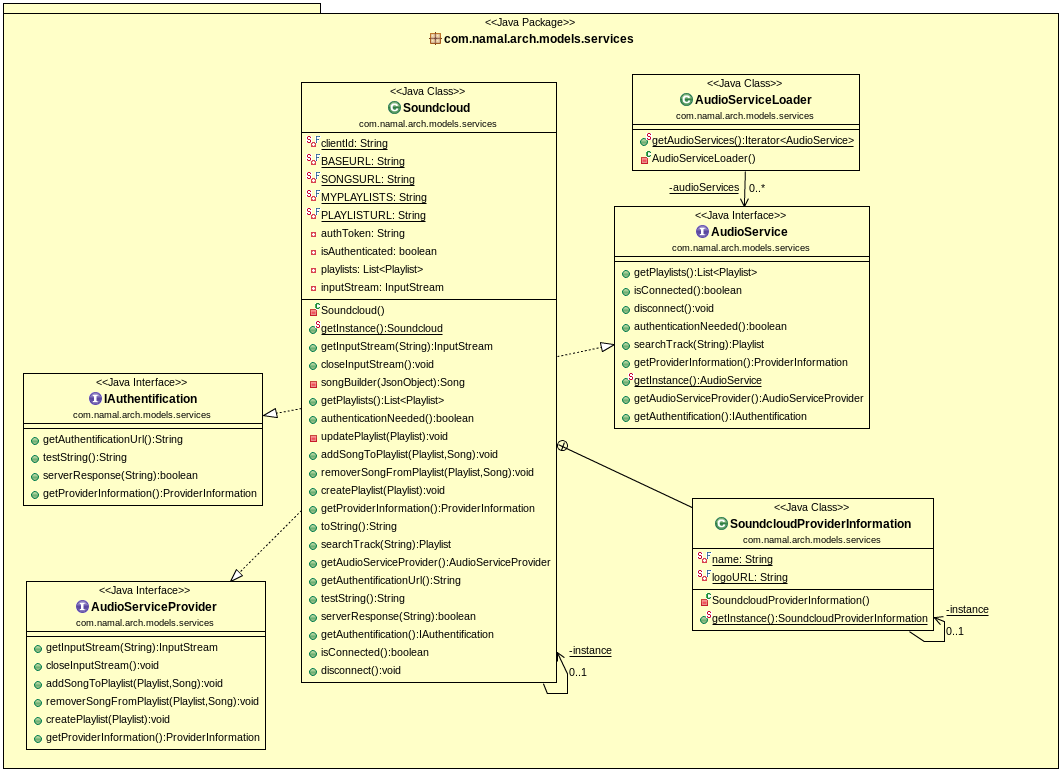
\includegraphics[scale=0.4]{class/Services.png}
  \caption{Former Services package diagram}
  \label{UpdateFormerServices}
\end{figure}

\begin{figure}[H]

  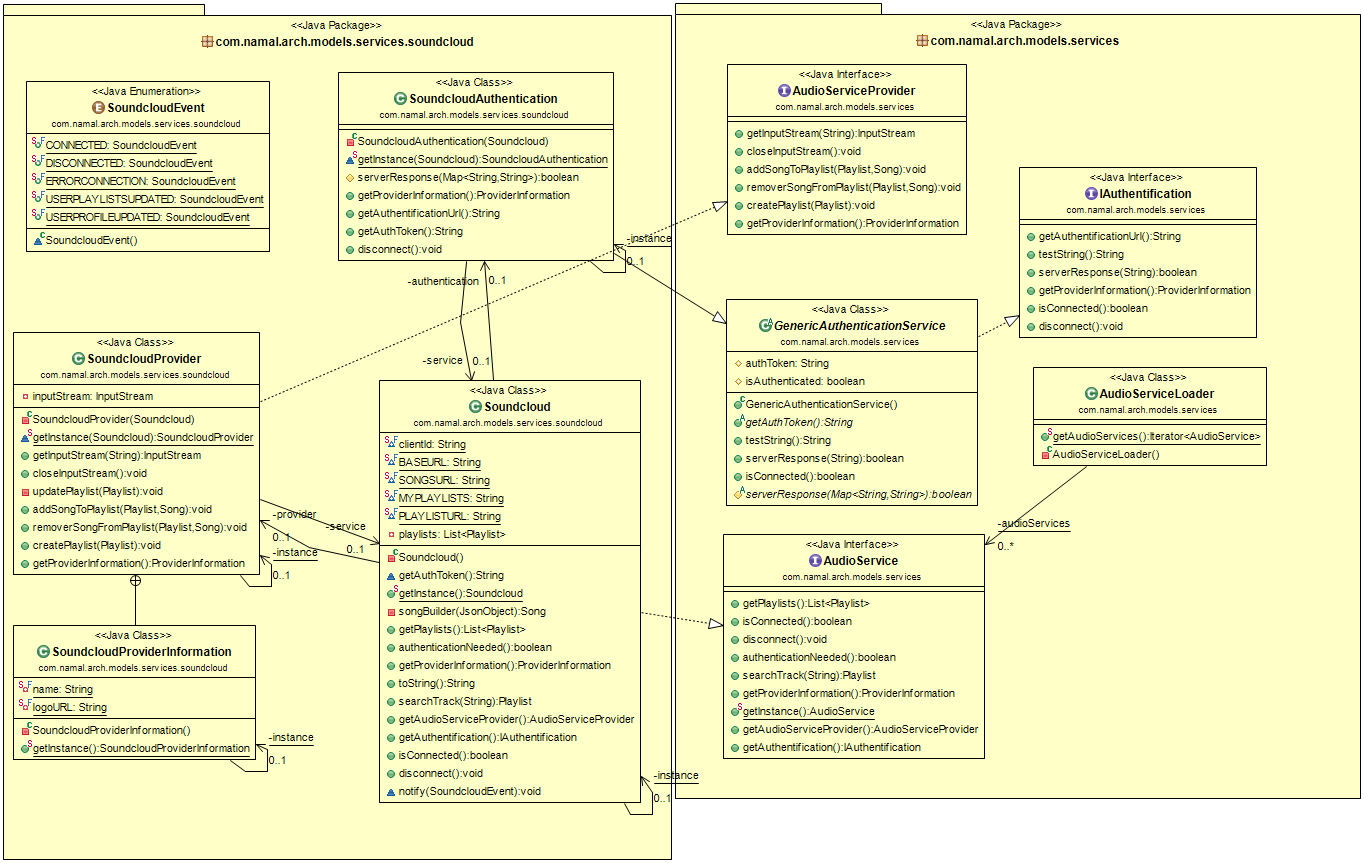
\includegraphics[scale=0.4]{class/Services2.png}
  \caption{New Services package diagram, including the SoundCloud package.}
  \label{UpdateServices}
\end{figure}
}

\subsubsection{Explanations}
The \texttt{Soundcloud} class was implementing on its own three interfaces, ie at least three different responsibilities. In detail, the \texttt{Soundcloud} class was managing the authentication, the audio service, and was an audio service provider at the same time. The authentication on Soundcloud follows a quite common process, which is also used with many other providers. It was then easier to create a new class \texttt{GenericAuthenticationService}, which enabled to define standard methods used in the authentication process of the providers, and give the responsibility of dealing with the authentication on Soundcloud to one dedicated class (the \texttt{SoundcloudAuthentication} class) who inherits the \texttt{GenericAuthenticationService} class. \\
An enumeration has been created to make the type of the Soundcloud event easier to manipulate.\\
A class defining the behaviour of \texttt{AudioServiceProvider} of Soundcloud has also been created to separate the actions that can be performed (as a provider of services) from  the representation of Soundcloud as a service inside the software. Indeed, the \texttt{Soundcloud} class is supposed to represent one of the web-services the software handles and not a direct interface to the Soundcloud API.

\subsection{JavaDoc}
The group who reviewed our project suggested us to make a more comprehensive Java Documentation, we tried to improve the Java Documentation available into our source code. We hope that we managed to improve it, even if it remains very subjective.

\subsection{Other recommendations}
The other group also advised us to split the \texttt{PlayerController} class, as it could be seen as a "God Class" with too many responsibilities. We took this suggestion into account, of course, but we went to the conclusion that it would maybe not be as suitable as it was for the \texttt{Soundcloud} class. Here is the explanation :

\begin{itemize}
\item The \texttt{PlayerController} is made of two major parts : the Observer pattern, as a subject of some View and as an observer of the \texttt{PausablePlayer}, and the player controlling methods.
\item The Observer pattern cannot be split or implemented on another class, because it needs to be able to  observe the \texttt{PausablePlayer} and transmit this observation to the view, while updating its own state.
\item All the other methods have the responsibility to manage the state of the controller but also of the \texttt{PausablePlayer}, the concrete implementation of the music player. Some of them give feedbacks to the view of the current state of the music player, but they have a quite high cohesion and would be hard to split into two classes.
\item We could have managed the current song index and similar matters directly into the \texttt{Playlist} class, but we wanted to keep the \texttt{Playlist} class as a data structure to encapsulate a list of songs, with limited responsibilities otherwise than giving easier access through appropriate getters and setters.
\end{itemize}
}

\ifthenelse{\boolean{lab2} \OR \boolean{all}}{
\ifthenelse{\boolean{all}}{
\section{Laboratory n$\degree$2}}

For this laboratory we had an agreement with the laboratory teacher as to which features would be implemented :
\begin{itemize}
\item Add RCP/e4 buttons
\item Add Spotify and Deezer
\item Have a better Javadoc
\end{itemize}

We are proud to announce that not only have we added all those features, but we also added management of cross-platform playlists!

\subsection{Architecture}

The architecture hasn't been modified for the first 2 features. Indeed, for the first feature Fabien had already created the Observer in order for all observing views to be notified when the player changed state. We only had to add the buttons as observers. For the second feature, we added Spotify and Deezer without any trouble. The laboratory teacher assured us that our architecture wasn't good enough for more than one service (without any proof), but it works perfectly.

The architecture has however changed for cross-platform playlists. However, as \hyperlink{db}{we said previously}, the tweaks were minor. Here are the new class diagrams :

\iftoggle{diag}{
\begin{figure}[H]

  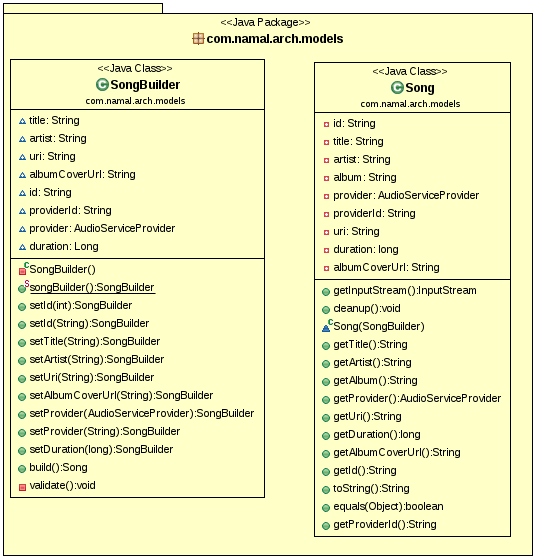
\includegraphics[scale=0.4]{class/update-2-1.png}
  \caption{Modified models}
  \label{modmod}
\end{figure}

\begin{figure}[H]

  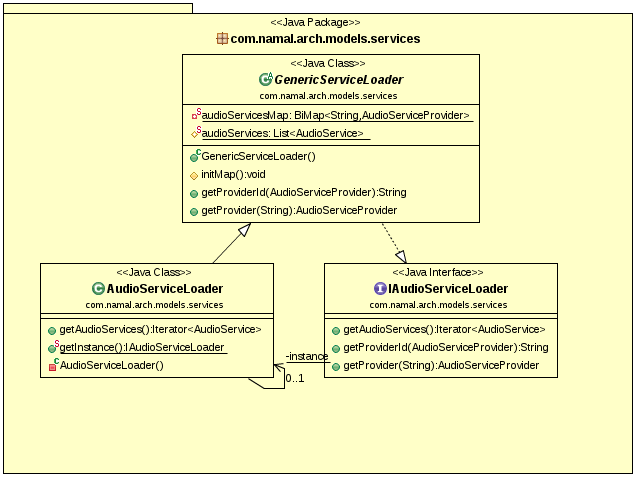
\includegraphics[scale=0.4]{class/update-2-2.png}
  \caption{Modified service loaders}
  \label{modSL}
\end{figure}
}

The modifications are primarily because we had to save not the AudioServiceProvider but an ID of said Provider. The link between the services and the ID are in the database. For now, we have manually added the services and their IDs to the database. In the third laboratory, our server will create the ID if needed.

\subsection{RCP/e4 buttons}

The buttons were added without much trouble. All views are synchronized, ie. if the JavaFx view clicks on pause, the play button will transform to a pause button. This shows that our architecture was already robust enough for multiple views.

\subsection{MongoDB}

We decided to use a database anticipating the third laboratory (instead of saving the playlist in a local file for instance). We went with MongoDB because it's easy to use and modern. Furthermore, you can create an online database for testing for free (MongoLab). It allows us to test our application in \textit{real-life} conditions. 

\subsection{New bugs}

A known bug that has been introduced with cross-platform playlist is that if a ServiceProvider is unavailable, say Spotify, and a playlist has a Spotify song, when you try and open said playlist, and exception is thrown. This major bug will be fixed in time for the next laboratory.

\subsection{Javadoc}

We added the necessary Javadoc to the first and second laboratory.

\subsection{Other recommendations}

Due to a lack of time, we weren't able to consider the suggestions of our colleagues -except those that were the same as our objectives-, especially given the fact that they weren't major architecture flaws/bugs. Indeed, we focused on the agreement we had with the laboratory teacher. However, we have saved those suggestions and hope to have enough time to add those features soon.

}


\end{document}